\documentclass{beamer} 
\usepackage{amsmath,amsthm}
\usepackage{mathrsfs}
\usepackage{amssymb}
\usepackage[english]{babel}
\usepackage{latexsym}
\usepackage{amsfonts}
\usepackage{graphicx}
\usepackage{float}
\usepackage{graphics}
\usepackage{epsfig}
\usepackage{url}
\usepackage{soul}
\usepackage{listings}
\usepackage{bm}
\usepackage{braket}

% \usepackage{minted}


\usetheme{WVU}
\usecolortheme{WVU}
\usepackage{multirow}

\mode<presentation> 

\title[VE401 SU2022 RC week11]{VE401 SU2022 RC week11}

\author[ Shuyu Wu ]{ Shuyu Wu }
\institute[UM-SJTU JI]{UM-SJTU Joint Institute \vspace{.2cm} \\ 
\includegraphics[scale=0.3]{umji_logo.png}\\wushuyu2002@sjtu.edu.cn}
\date[July 2022]{\today}

\begin{document}
\begin{frame} 

\titlepage 

\end{frame} 

\section{Next Week's Plan}
\begin{frame}
    \frametitle{Outline}
    \tableofcontents[currentsection]
\end{frame}

\begin{frame}
    \frametitle{Next Week's Plan}
    \begin{itemize}
        \item July 27: (probably) no RC for another TA.
        \item July 30: my regular RC hold as usual, but with different style
        \item July 31: big RC
        \item August 1: final exam, and end of the course for you (not for me)
    \end{itemize}
    
\end{frame}

\begin{frame}
    \frametitle{My Next Week's RC On July 30}

    This is an onsite evaluation leaded by The Center for Learning and Teaching (CLT) for me to get advanced TA certificate. Some TA mentors will come and watch.\par
    \vspace{0.3cm}
    The teaching language will be English, of course. There will be many interactions between the TA (me) and you, which is called ``active learning''.\par
    \vspace{0.3cm}
    Please do me some favor and come if you can. Interaction is much appreciated!

\end{frame}

\begin{frame}
    \frametitle{Recap}

    \begin{itemize}
        \item calculation of model parameters
        \item matlab curve fitting toolbox
        \item some problems in assignment 9
    \end{itemize}

\end{frame}

\section{Simple Linear Regression II:
Predictions and Model Analysis}
\begin{frame}
    \frametitle{Outline}
    \tableofcontents[currentsection]
\end{frame}
\begin{frame}
    \frametitle{Inferences about a Single Predicted Value}

    Confidence Interval the Estimated Mean $\mu_{Y|x}$: 
    \[\hat{\mu}_{Y|x}\pm t_{\alpha/2, n-2}S\sqrt{\frac{1}{n}+\frac{(x-\overline{x})}{S_{xx}}}\]
    Please notice that $\mu_{Y|x}$ is a parameter, not a random variable.\par
    Now we want to know what we will get for $Y|x$ next time we get X=x, which is a random variable. That is to say, we want the prediction of the random variable.\par
    The $100(1-\alpha)\%$ prediction interval for $Y|x$ is given by
    \[\widehat{Y|x}\pm t_{\alpha/2, n-2}S\sqrt{1+\frac{1}{n}+\frac{(x-\overline{x})}{S_{xx}}}\]
    The $\widehat{Y|x}=\hat{\mu}_{Y|x}=b_0+b_1 x$

\end{frame}

\begin{frame}
    \frametitle{Coefficient of Determination $(R^2)$}

    $SS_{T}:=S_{yy}$ is the Total Sum of Squares. $SS_{E}:=\sum\limits_{i=1}^{n} e_i^2=\sum\limits_{i=1}^{n} (y_i-(b_0+b_1 x))^2$ represents the variation of Y that remains after we have applied the
    model.\par
    \[R^2:=1-\frac{SS_{E}}{SS_{T}}\]
    Also we have 
    \[R^2=\frac{S_{xy}^2}{S_{xx}S_{yy}}\]

\end{frame}

\begin{frame}
    \frametitle{Significance of Regression}

    \[T_{n-2}=\frac{R}{\sqrt{1-R^2}}\sqrt{n-2}\]
    This is a two-tailed test. And we do not need $S^2$, $SS_{E}$ or $S_{xx}$ now.\par
    Or we can use F-test (which can be generalized to multiple linear regression).\par
    \[F_{1,n-2}=(n-2)\frac{R^2}{1-R^2}=(n-2)\frac{SS_{T}-SS_{E}}{SS_{E}}\]
    Reject $H_0: \beta_1=0$ at significance level $\alpha$ when $F_{1,n-2}>f_{\alpha,1, n-2}$. Note that this is a one-tailed test.\par
    Since $R$ means correlation, we can use the T-test to test bivariate normal distribution with correlation coefficient $\rho$ for $H_0: \rho=0$
\end{frame}

\begin{frame}
    \frametitle{Lack-of-Fit and Pure Error}

    When we get a low $R^2$ (or big $SS_{E}$), two reason for that: the $\sigma$ of the noise term is large, or the model is wrong. \par
    Method: repeat test for the same $x_i$.\par
    Let $Y_{ij}$ denote the jth observation of $Y|x_i$, where $j=1,2,\dots , n_i$. So total measurements is $n=\sum\limits_{i=1}^{k} n_i$. k is the number of different $x_i$.\par
    Internal sum of square for $\mu_{Y|x_i}$: $\sum\limits_{j=1}^{n_i}(Y_{ij}-\overline{Y_i})^2$

\end{frame}

\begin{frame}
    \frametitle{Lack-of-Fit and Pure Error}

    Sum up all the internal sum of square, we get the error sum of squares due to pure error, $SS_{E;pe}$.\par
    \[SS_{E;pe}:=\sum\limits_{i=1}^{k}\sum\limits_{j=1}^{n_i}(Y_{ij}-\overline{Y_i})^2\]
    And $\frac{SS_{E;pe}}{\sigma^2}$ follows $\chi^2_{n-k}$. Also $SS_{E;lf}$ (the error sum of squares due to lack of fit) is defined as
    \[SS_{E;lf}:=SS_E-SS_{E;pe}\]
    And $\frac{SS_{E;lf}}{\sigma^2}$ follows $\chi^2_{k-2}$.

\end{frame}

\begin{frame}
    \frametitle{Testing for Lack of Fit}

    Then divide them and we expect an F distribution. We have 
    \[F_{k-2,n-k}=\frac{SS_{E;lf}/(k-2)}{SS_{E;pe}/(n-k)}\]
    And reject $H_0: \text{the model is proper}$ at significance level $\alpha$ when $F_{k-2,n-k}>f_{\alpha,k-2,n-k}$.

\end{frame}

\section{Multiple Linear Regression I: Basic Model}
\begin{frame}
    \frametitle{Outline}
    \tableofcontents[currentsection]
\end{frame}


\begin{frame}
    \frametitle{Generalized Regression Models}
    \begin{enumerate}
        \item Generalize the number of variables
        \[\mu_{Y|x_1\dots x_p}=\beta_0+\beta_1 x_1+\dots +\beta_p x_p\]
        \item Generalize the degree of the polynomial
        \[\mu_{Y|x}=\beta_0+\beta_1 x+\dots +\beta_p x^p\]
        \item Mixture, for example, 
        \[\mu_{Y|x_1\dots x_p}=\beta_0+\beta_1 x_1+\beta_2 x_2+\beta_3 x_1 x_2\]
    \end{enumerate}
    These are all called \textbf{Multiple Linear Regression}, and we have a set of general theory to tackle these problems.\par
    Question: Why 2 and 3 are also called ``linear''?
    

\end{frame}

\begin{frame}
    \frametitle{The Polynomial Model}

    We first talk about Polynomial Model.\par
    Suppose we have a set of n sample, $(x_i,y_i)$, $i=1,2,\dots , n$. Our goal is to find the estimate of $\beta_0$ to $\beta_p$, denoted as $b_0, \dots , b_p$, such that
    \[y_i=b_0+b_1 x_{i}^1+\dots +b_p x_i^p+e_i\]
    And the sum of squares error, 
    \[SS_{E}=\sum\limits_{i=1}^{n} e_i^2\]
    is minimized.

\end{frame}

\begin{frame}
    \frametitle{The Model Specification Matrix}

    For the model $Y_i=\beta_0+\beta_1 x_i+\dots +\beta_p x_i^p + E_i$, $i=1,2,\dots , n$, we can use a matrix equation to represent
    \[\mathbf{Y}=X\boldsymbol{\beta}+\mathbf{E}\]
    And 
    \begin{equation*}      
        \mathbf{Y}=
        \left( 
          \begin{array}{ccc}  
        
            Y_1\\
            \vdots\\
            Y_n
          \end{array}
        \right)   
        , X=
        \left(
        \begin{array}{ccccc}
            1 & x_1 & x_1^2 & \cdots & x_1^p\\
            \vdots & \vdots & \vdots & \ddots & \vdots\\
            1 & x_n & x_n^2 & \cdots & x_n^p
        \end{array}
        \right)
        , \mathbf{E}=
        \left(
            \begin{array}{ccc}  
        
                E_1\\
                \vdots\\
                E_n
              \end{array}
        \right)
    \end{equation*}
    The $X$ is called the model specification matrix. Each row is one sample, and each column coresponds to one term in the model.

\end{frame}

\begin{frame}
    \frametitle{ex 11.1}

    Write down the model specification matrix for the other two models in page 3.
    \[\mu_{Y|x_1\dots x_p}=\beta_0+\beta_1 x_1+\dots +\beta_p x_p\]

    \[\mu_{Y|x_1\dots x_p}=\beta_0+\beta_1 x_1+\beta_2 x_2+\beta_3 x_1 x_2\]

\end{frame}

\begin{frame}
    \frametitle{ex 11.1 answer}
    Question 1: denote $x_{ij}$ as the jth sample of $x_i$, we have
    \begin{equation*}
        X=
        \left(
        \begin{array}{ccccc}
            1 & x_{11} & x_{21} & \cdots & x_{p1}\\
            \vdots & \vdots & \vdots & \ddots & \vdots\\
            1 & x_{1n} & x_{2n} & \cdots & x_{pn}
        \end{array}
        \right)
    \end{equation*}
    Question 2: denote $x_{ij}$ as the jth sample of $x_i$, we have
    \begin{equation*}
        X=
        \left(
        \begin{array}{ccccc}
            1 & x_{11} & x_{21}  & x_{11}x_{21}\\
            \vdots & \vdots & \vdots  & \vdots\\
            1 & x_{1n} & x_{2n}  & x_{1n}x_{2n}
        \end{array}
        \right)
    \end{equation*}

\end{frame}

\begin{frame}
    \frametitle{The Regression Coefficients}

    Now we want to calculate $\mathbf{b}$ which is the estimator of $\boldsymbol{\beta}$. Our result is
    \[\mathbf{b}=(X^{T}X)^{-1}X^{T}\mathbf{Y}\]
    Please notice that this applies to any linear regressions, not only for polynomial model.\par
    Of course, you'd better do the calculation with matlab or other softwares.

\end{frame}



\begin{frame}
    \frametitle{ex 11.2}

    Our model is $y=b_0+b_1 x+b_2 x^2$, and we get 10 samples. Please find $b_0, b_1, b_2$.\par
    x: 0.5    1.0    1.5    2.0    2.5    3.0    3.5    4.0    4.5    5.0\par
    y: 1.4135    3.8133    6.9435   11.3157   15.6289   20.0300   26.8820   33.1451   40.4624   48.8429

\end{frame}

\begin{frame}
    \frametitle{ex 12.2 answer}

    Method 1: Use matlab curve fitting app.\par
    \begin{figure}[H]
        \centering
        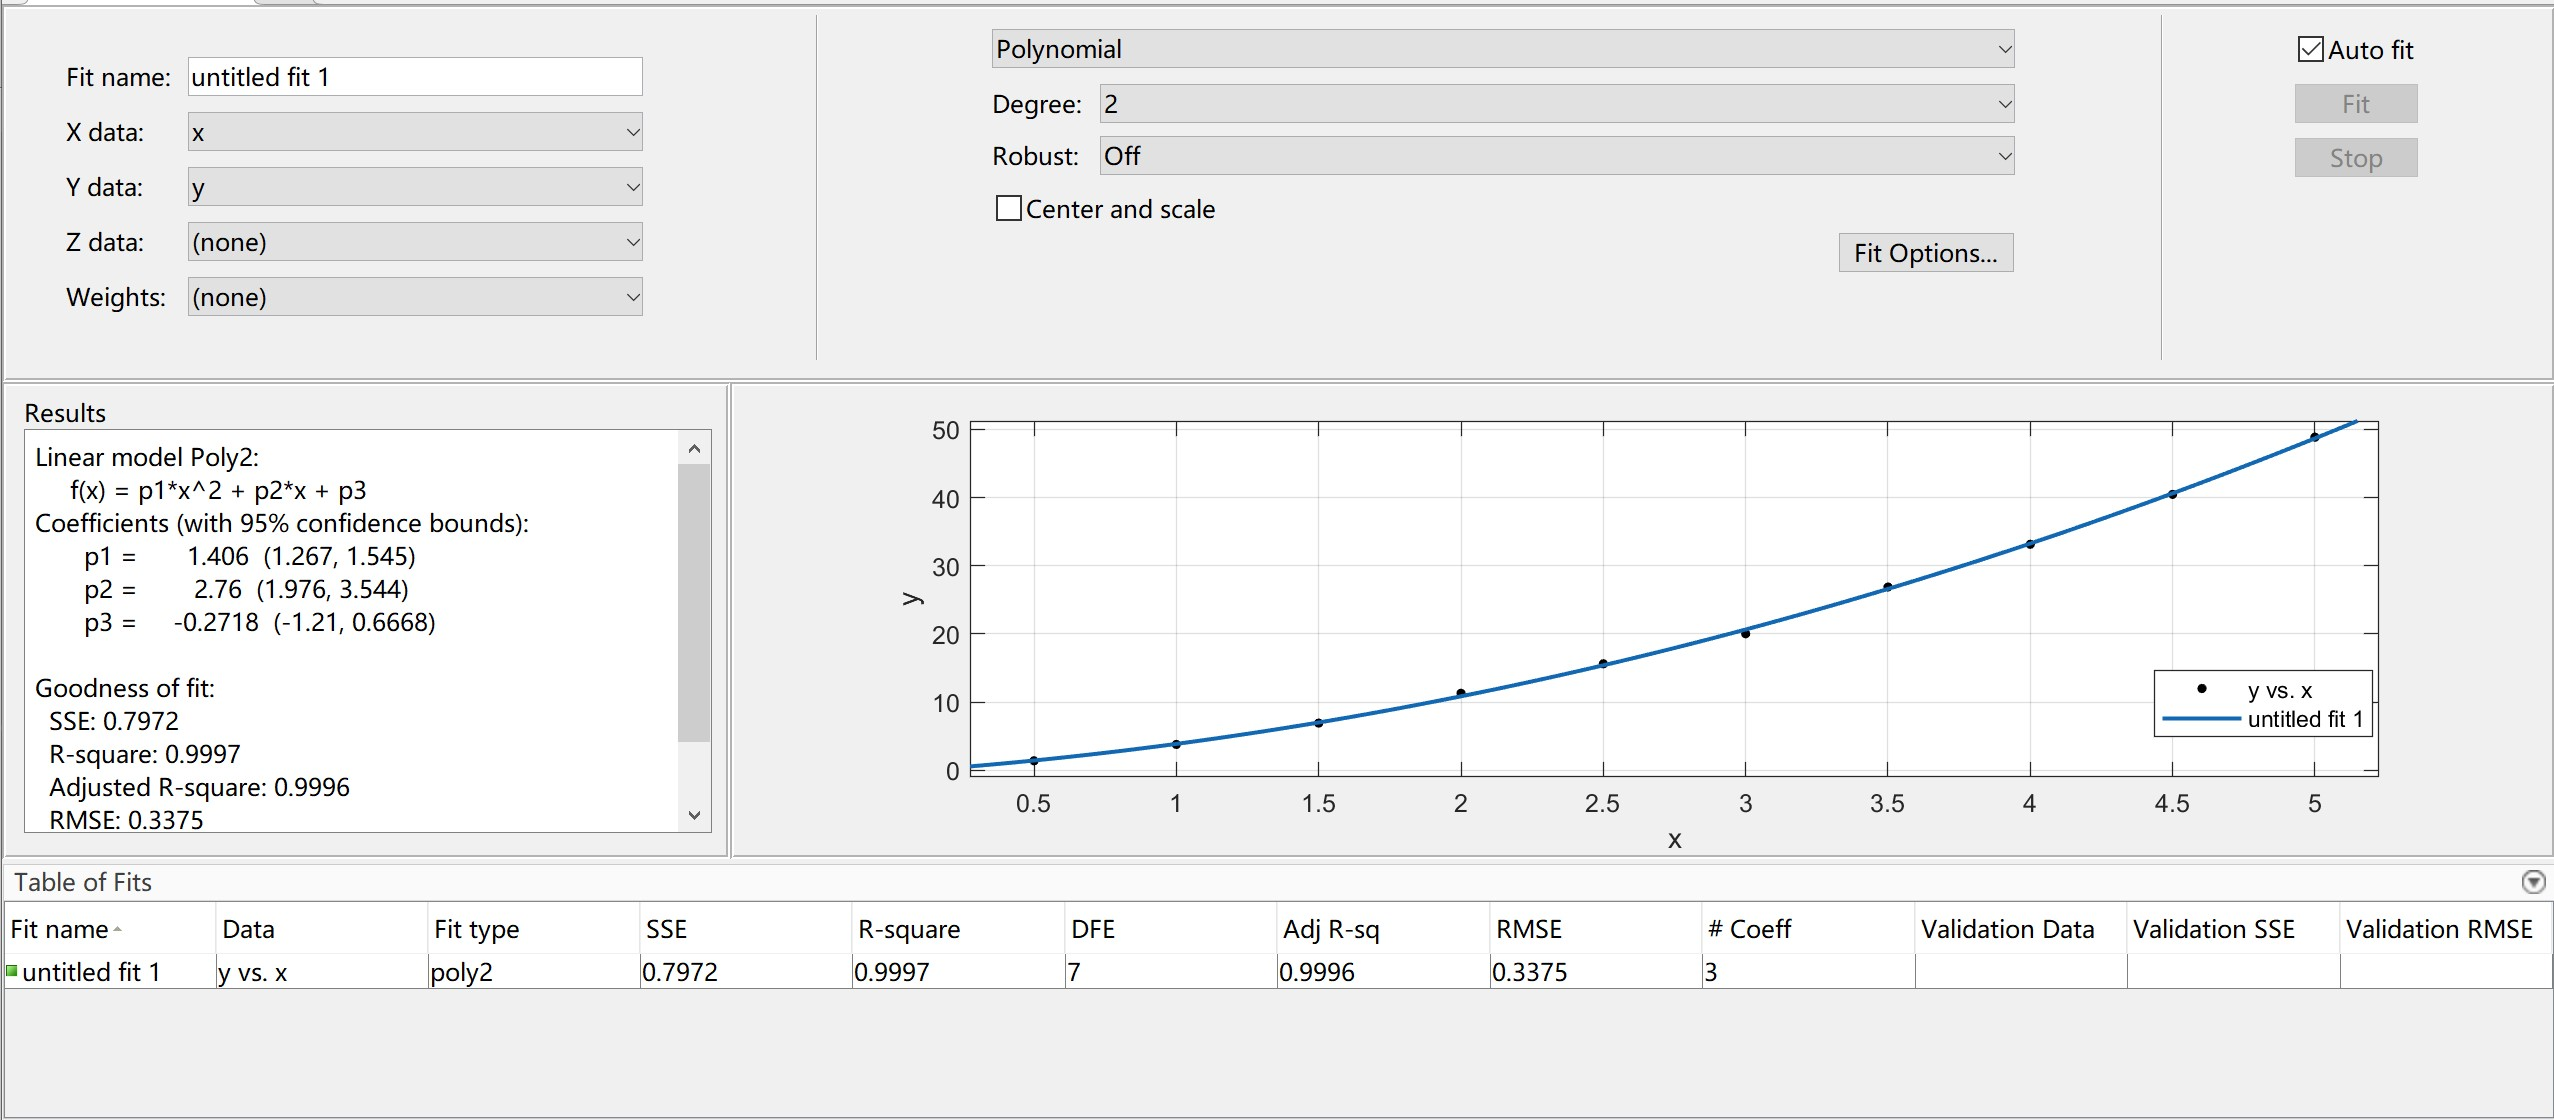
\includegraphics[width=0.6\textwidth,height=0.3\textwidth]{ex12_2_1.jpg}
        \caption{fitting result}
    \end{figure}\par
    We can directly read off the result: $b_2=1.406, b_1=2.76, b_0=-0.2718$. \par
    We can also get: $SS_{E}=0.7972, R^2=0.9997$.
\end{frame}

\begin{frame}
    \frametitle{ex 11.2 answer}
    Method 2: Direct calculation.
    \par
    \begin{figure}[H]
        \centering
        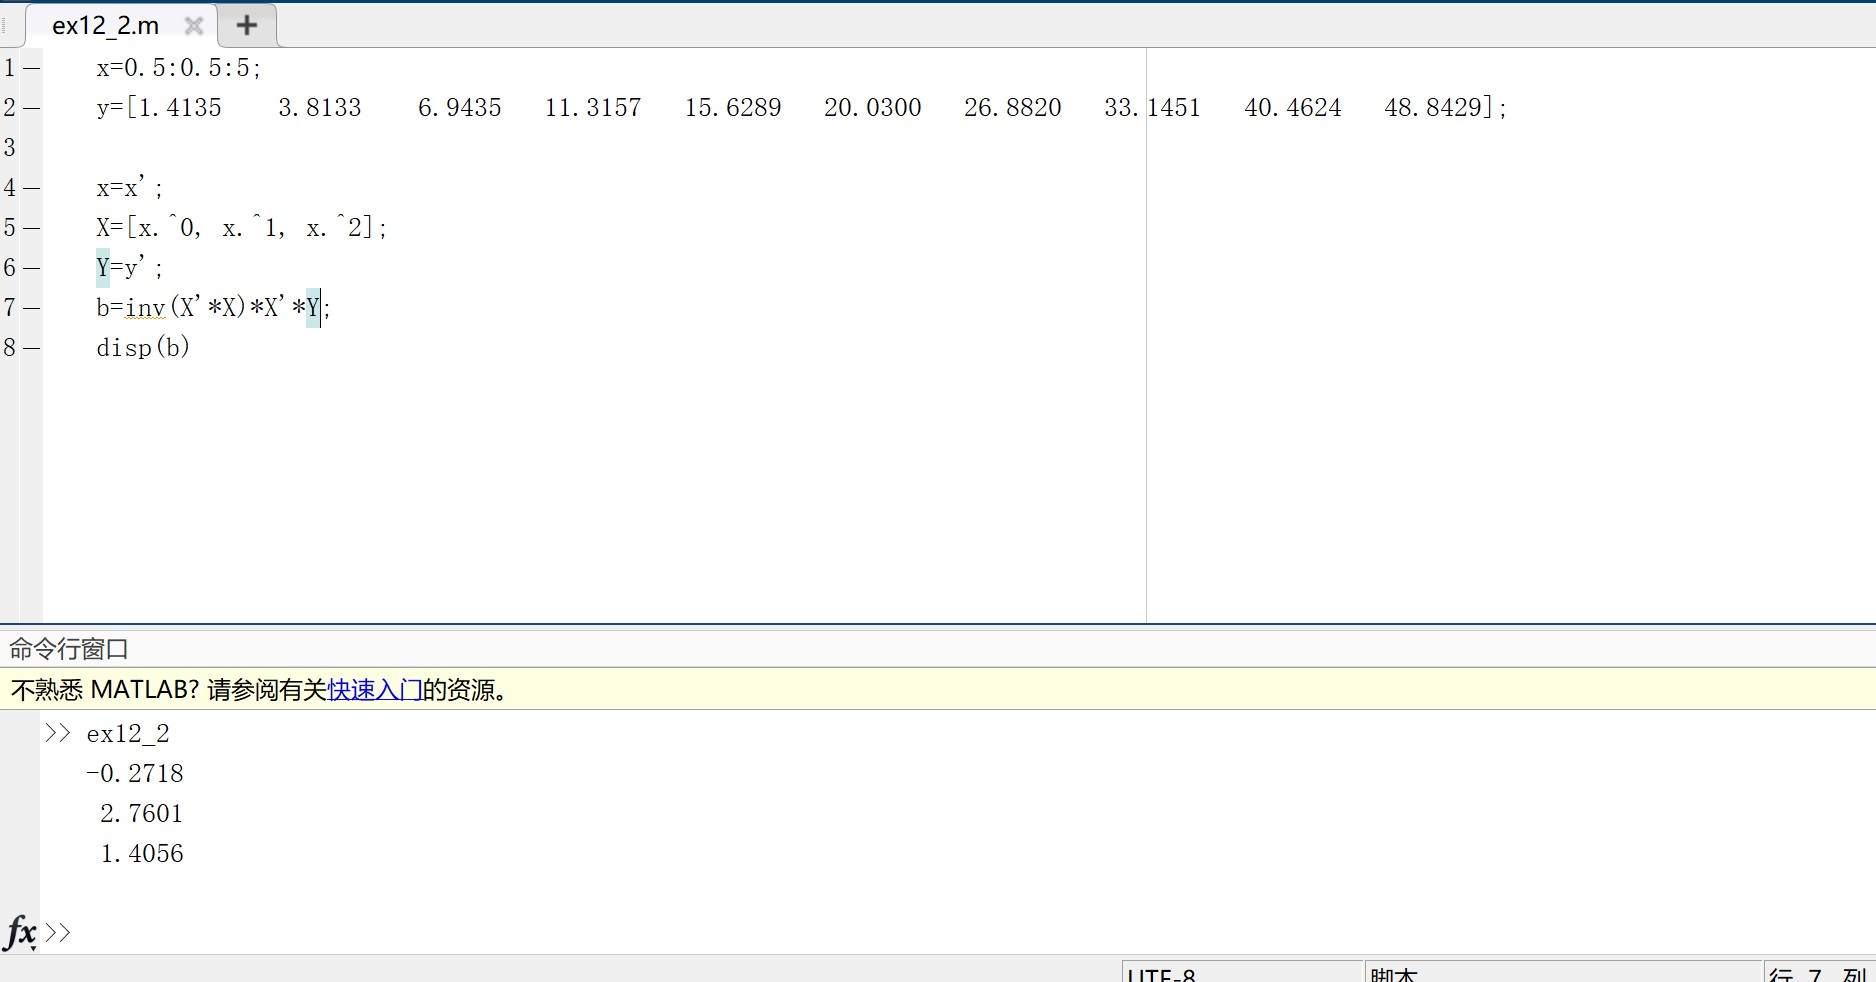
\includegraphics[width=0.6\textwidth,height=0.3\textwidth]{ex12_2_2.jpg}
        \caption{fitting result}
    \end{figure}\par
    We get basically the same result: $b_0=-0.2718, b_1=2.7601, b_2=1.4056$

\end{frame}

\begin{frame}
    \frametitle{The Multilinear Model}

    Basically the same thing. You need to use a different model specification matrix, which is
    \begin{equation*}
        X=
        \left(
        \begin{array}{ccccc}
            1 & x_{11} & x_{21} & \cdots & x_{p1}\\
            \vdots & \vdots & \vdots & \ddots & \vdots\\
            1 & x_{1n} & x_{2n} & \cdots & x_{pn}
        \end{array}
        \right)
    \end{equation*}
    And you can follow the same process.

\end{frame}

\begin{frame}
    \frametitle{Error Analysis}

    We want to measure $SS_{E}$ and $R^2$. You can of course get them from matlab, but you're recommended to also know how to calculate them directly.\par
    Like the simple linear regression, we need to analysis $SS_{T}$ and $SS_{E}$.
    \[SS_{T}=\sum\limits_{i=1}^{n}(Y_i-\overline{Y})^2, SS_{E}=||Y-Xb||^2\]


\end{frame}

\begin{frame}
    \frametitle{Error Analysis}

    The P projection is an $n*n$ matrix with value $\frac{1}{n}$ for each of the element. The hat matrix $H:=X(X^{T}X)^{-1}X^{T}$. Our result for $SS_{T}$ and $SS_{E}$ are:
    \[SS_{E}=\Braket{Y, (\mathbb{I}_{n}-H)Y}, \]
    \[SS_{T}=\Braket{Y,(\mathbb{I}_{n}-P)Y}=SS_{E}+SS_{R}\]
    \[R^2=1-\frac{SS_{E}}{SS_{T}}\]

\end{frame}

\begin{frame}
    \frametitle{ex 11.3}

    Calculate the $SS_E$ and $R^2$ in ex 12.2

\end{frame}

\begin{frame}
    \frametitle{ex 11.3 answer}

    \begin{figure}[H]
        \centering
        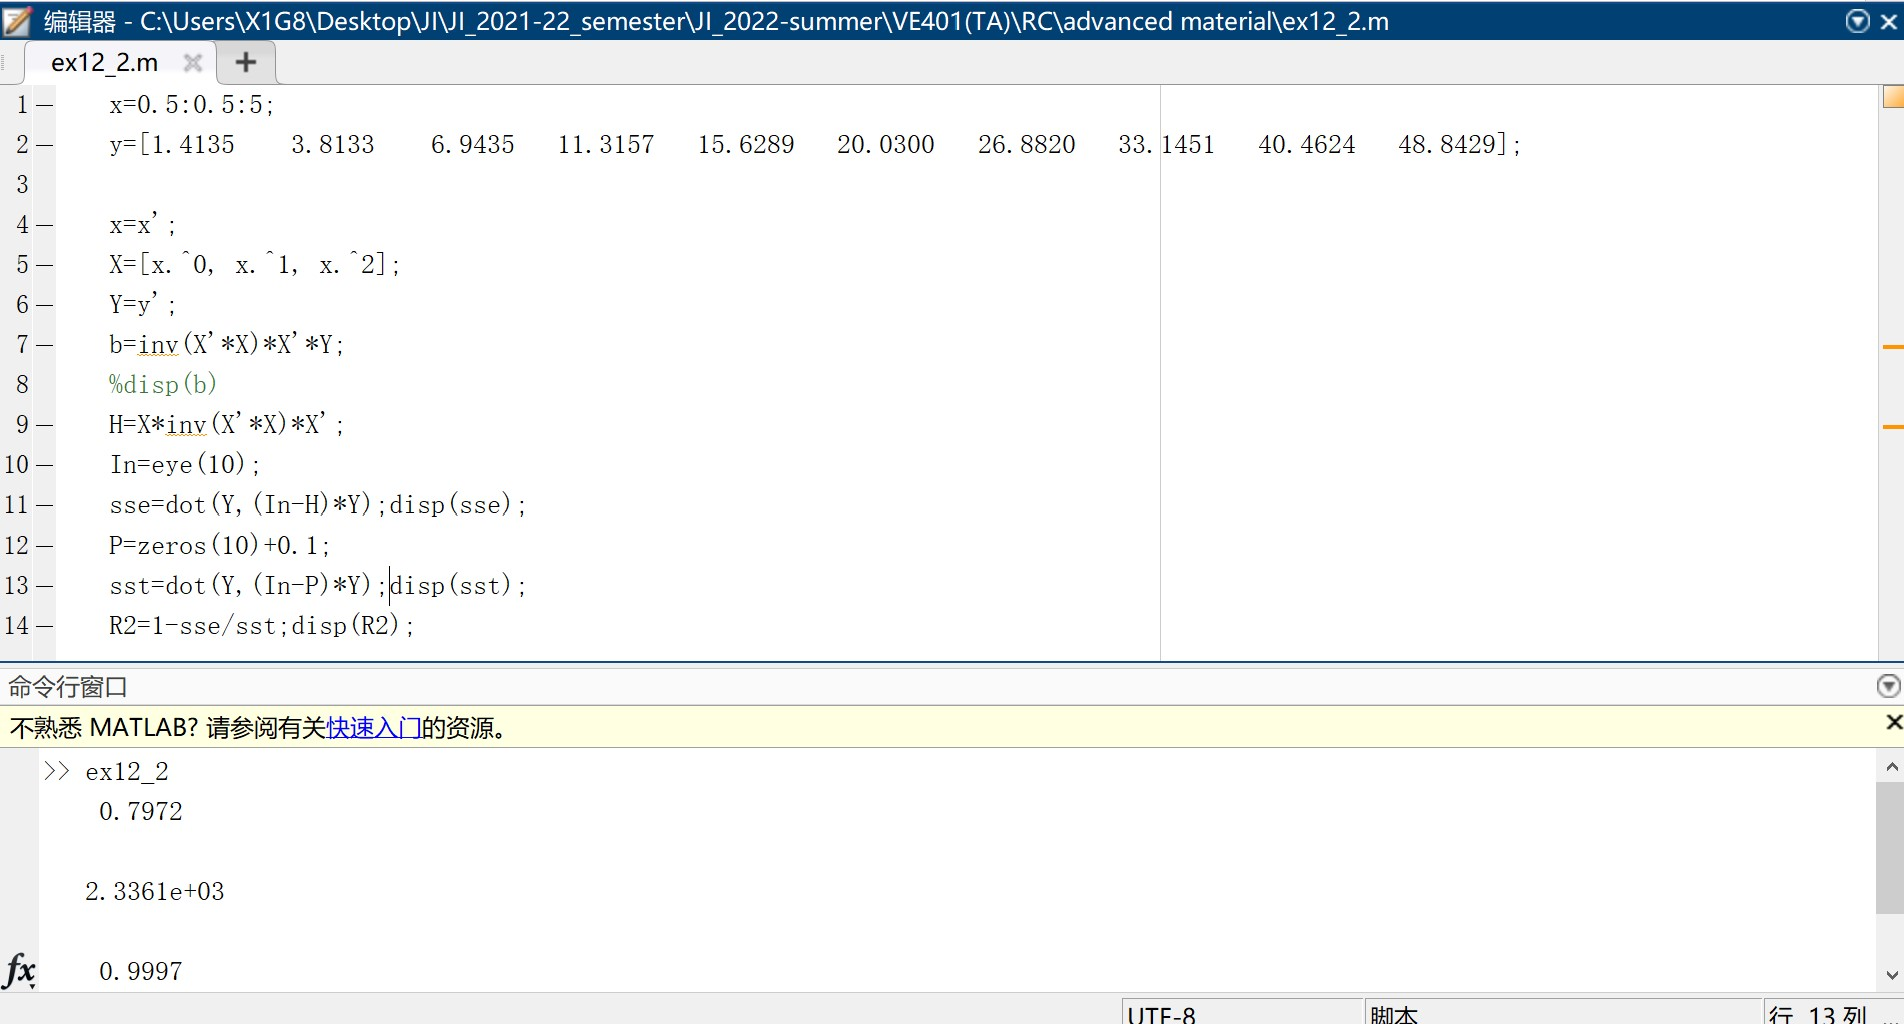
\includegraphics[width=0.6\textwidth,height=0.3\textwidth]{ex12_3.jpg}
        \caption{fitting result}
    \end{figure}\par
    The result is the same to ex12.2 when we use curve fitting toolbox: $SS_{E}=0.7972$, $R^2=0.9997$. Perfect!

\end{frame}



\section{Extra topic and Q\&A}
\begin{frame}
    \frametitle{Outline}
    \tableofcontents[currentsection]
\end{frame}

\begin{frame}
    \frametitle{Q\&A}
    
    Feel free to ask if you have any questions.\par
    
    
    
\end{frame}

\end{document} 